\label{Chapter3}

\chapter{Implementation and Tools}

\section{Planetary Rover Testbed} \label{hdpr_rover}

In order to benchmark our system in real scenarios, we implemented the
system in a testbed rover and integrated it with the rest of its components.
The rover we used is named Heavy Duty Planetary Rover (HDPR) and is
capable of traversing different types of terrain with a speed of up to
$\SI{1}{\m \per sec}$.
It was developed by the Automation and Robotics Lab (ARL/TEC-MMA) of the
European Space Agency (ESA) and is currently used for validating
software and hardware components in long range scenarios.

The HDPR rover, depicted in Figure \ref{fig:hdpr_rover}, bears close
resemblance to the camera setup of the ExoMars mission rover and allows the
evaluation of algorithms that have a focus on autonomous navigation.
Specifically, the sensor suite of the rover comprises of the following
components:

\begin{figure}[h!]
    \centering
    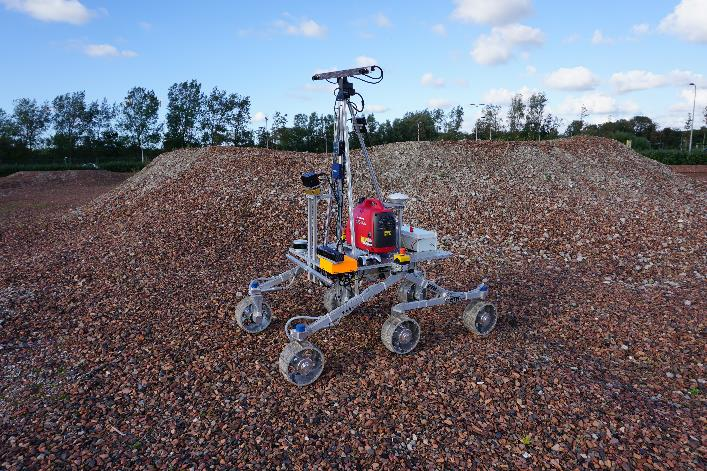
\includegraphics[scale=0.5]{hdpr_rover}
    \decoRule
    \caption[Heavy duty planetary rover]{
        The Heavy duty planetary rover (HDPR).
    }
    \label{fig:hdpr_rover}
\end{figure}

\begin{itemize}
    \item Exteroceptive:
        \begin{itemize}
            \item LocCam stereo camera (PointGrey Bumblebee 2)
            \item PanCam stereo camera (PointGrey Grasshoper 2)
            \item Kinect time of flight camera
            \item MESA SR4500 time of flight camera
            \item Velodyne LiDAR (VLP-16)
        \end{itemize}
    \item Proprioceptive:
        \begin{itemize}
            \item Trimble GNSS receiver (BD970)
            \item Inertial Measurement Unit (Sensonor STIM300)
            \item Shaft Encoders and Potentiometers
        \end{itemize}
\end{itemize}

From these sensors, we exploit
\begin{enumerate*}[label=(\roman*)]
    \item the LocCam for visual odometry inputs and
    \item the PanCam for SLAM inputs.
\end{enumerate*}
The LocCam has a baseline of $\SI{120}{\mm}$, is positioned about
$\SI{1.1}{\m}$ above the ground and is tilted at an angle of $18^{\circ}$.
The PanCam has a baseline of $\SI{500}{\mm}$, is positioned about
$\SI{1.9}{\m}$ above the ground, is tilted at an angle of $19^{\circ}$ and
has a field of view (FoV) of $40^{\circ}$.

In addition, the Inertial Measurement Unit (IMU) provides measurements about
the orientation and acceleration of the robot.
Although the rest of the sensors are not actively used by our system,
they can be exploited for validation purposes.

% TODO(ref): HDPR paper

\section{Overall System Architecture}

As we mentioned previously, the GA SLAM system was designed to function
with point cloud based inputs in addition to odometry inputs.

To utilize the sensor suite of the HDPR rover, we can extract point clouds
using stereo processing techniques and odometry estimation using visual
odometry methods.
For the former we employ the PanCam stereo camera and for the latter we make
use of the LocCam stereo camera.
Furthermore, we exploit the measurements received from the IMU to augment
the estimation of the robot's pose.
The utilization of each sensor of the HDPR rover w.r.t. to our system,
is shown in the system component diagram of Figure
\ref{fig:system_component_diagram}.

\begin{figure}[h!]
    \centering
    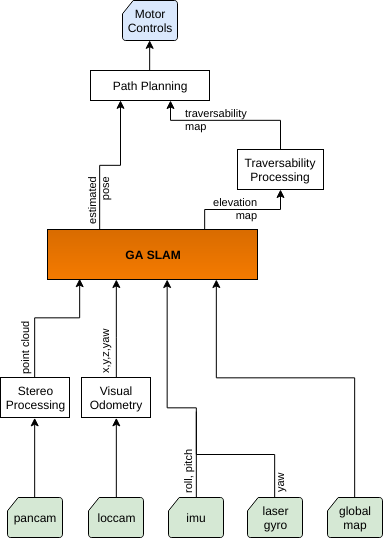
\includegraphics[scale=0.7]{system_component_diagram}
    \decoRule
    \caption[System component diagram]{
        The components of the system that enable the HDPR to perform
        autonomous navigation tasks.
    }
    \label{fig:system_component_diagram}
\end{figure}

As depicted, the local elevation map of the GA SLAM subsystem can be used
in order to extract a map that contains traversability features about the
surrounding environment of the rover, i.e. features that determine if
the rover is able to traverse a specific area.
At a next layer, the traversability map and the estimated pose from SLAM
can be utilized by a path planning module, with the aim to provide
autonomously control the rover in an unknown environment.
Finally, It should be noted that the choice of visual odometry
instead of plain wheel odometry, comes from the fact that a robot is prone
to slippage in outdoor environments, and more specifically planetary terrains.

\section{Library}

\subsection{Robotic Software Framework}

The GA SLAM system was implemented as a framework-independent library for C++
and depends only on libraries for linear algebra, point cloud processing
and image processing.
% TODO(ref): github repo
However, with the aim to provide integration with the rest of HDPR's
software modules and tools, we developed a component to bridge
the library using the Robot Construction Toolkit (ROCK).
% TODO(ref): Rock website

ROCK is a software framework for the development of robotic systems,
similar to Robot Operating System (ROS).
It differs from ROS in the sense that the development of applications
is achieved using a model driven approach.
It is implemented on top of the Orocos Real-Time Toolkit (Orocos RTT)
component layer and can provide real-time capabilities to a system.
In addition, it contains a rich collection of reliable and extensible
modules that are ready to use as well as tools for visualization and
task monitoring.

In ROCK, each distinct functionality of the system is
encapsulated in an RTT component (Figure \ref{fig:rock_component}) using a
tool called oroGen.
This tool, auto-generates the C++ code of the component, given
the specification of the component's interface.
The communication with the rest of the ROCK universe, is implemented through
a network of connected components.
This is achieved using the framework's Ruby modules which support the explicit
interconnection of a component's input port(s) with the output port(s)
of another component.

\begin{figure}[h!]
    \centering
    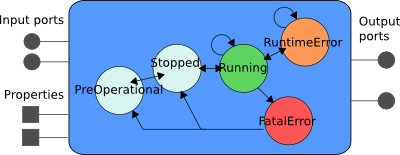
\includegraphics[scale=0.7]{rock_component}
    \decoRule
    \caption[ROCK component interface]{
        The interface and the state machine of a component in the Orocos
        Real-Time Toolkit. The output port(s) of a component can be explicitly
        connected to the input port(s) of another component. The properties
        are used to configure the component internally.
    }
    \label{fig:rock_component}
\end{figure}

% TODO(ref): Rock paper

\subsection{Orbiter Data Preprocessing}

As a means to validate the map matching capabilities of the system,
an orbiter (global) map is necessary.
A real example of such map has beeen reconstructed using orbital imagery,
depicted in Figure \ref{fig:hirise_map}, that was captured using the
High Resolution Imaging Science Experiment (HiRISE) camera mounted
on NASA's Mars Reconnaissance Orbiter (MRO).

It is possible to emulate an orbiter map using drone imagery.
The aerial images can then be used to reconstruct and provide a 3D
representation of the captured scene in the form of a densified point cloud.
At a later stage, the constructed point cloud can be projected in a 2D
grid and create an elevation map.

\begin{figure}[h!]
    \centering
    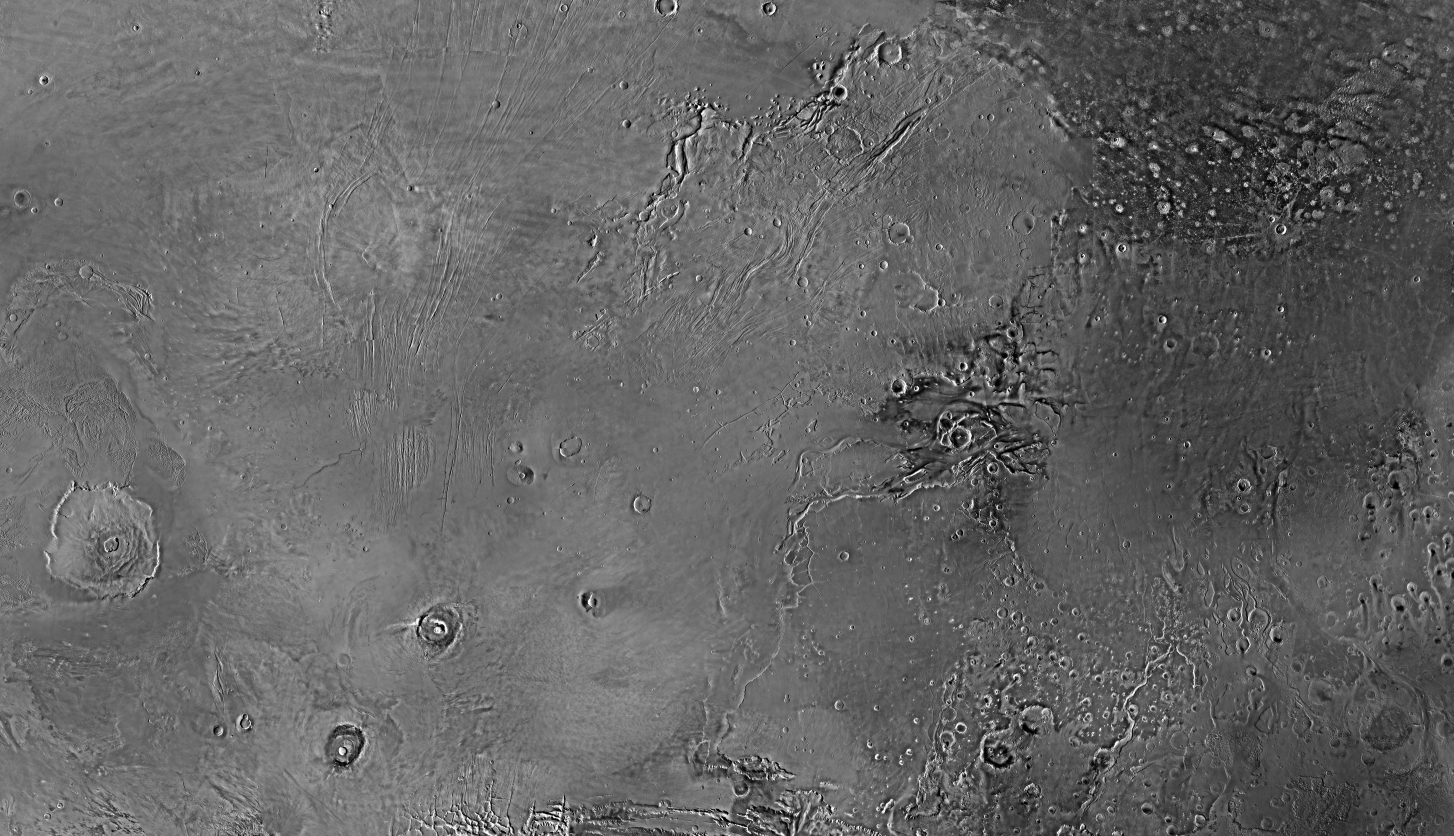
\includegraphics[scale=0.25]{hirise_map}
    \decoRule
    \caption[MARS view from HiRISE]{
        Close view of MARS that was captured using the HiRISE camera
        mounted on the Mars Reconnaissance Orbiter.
    }
    \label{fig:hirise_map}
\end{figure}

Prior to the projection, it is necessary to preprocess the global point cloud
in order to simplify it and transform it to a known reference system.
This is achieved in 4 steps:
\begin{enumerate*}[label=(\roman*)]
    \item voxelize point cloud to the desired resolution
    \item crop the voxel grid in the order of magnitude as the local map's
        size instead of using the whole information
        (e.g. for a local map of $\SI{10 x 10}{\m}$ crop the grid to
        $\SI{100 x 100}{\m}$)
    \item smooth the voxel grid using a Statistical Outlier Removal (SOR)
        filter which rejects points that are far from their neighbors
    \item transform the voxel grid to the robot's initial absolute pose.
\end{enumerate*}

% TODO: add figures of orbiter point cloud and the orbiter map

